\chapter{Sistema de Informação}
\label{sec:si}


\begin{overview}
  \lipsum[1]
\end{overview}


% \begin{figure}[!ht]
%   \caption{Componentes do Sistema de Informação}
%   \label{fig:flow-aquisicao}
%   \begin{center}
%     \smartdiagramset{set color list={orange!60,green!50!lime!60,
%           blue!50!cyan!70!white},
%       % planet color=orange!60,
%       planet size=2.6cm,
%       planet text width=2.6cm,
%       distance planet-satellite=4.0cm,
%       satellite size=3cm,
%       satellite text width=3cm,
%       % uniform connection color=true
%     }
%     \smartdiagram[connected constellation diagram]{
%       Sistema de\\Informação,Base de Dados\\(Seção \ref{sec:si-db}),FrontEnd\\(Seção \ref{sec:si-frontend}),Backend\\(Seção \ref{sec:si-backend})
%     }
%   \end{center}
% \end{figure}
Nesta seção, será descrito desenvolvimento do sistema de informação, esboçado na Fig. \ref{fig:si}, composto por um banco de dados (Seção \ref{sec:si-db}), um backend (Seção \ref{sec:si-backend}) e um frontend (Seção \ref{sec:si-frontend}), que, juntos, são responsáveis pelo armazenamento, manipulação e recuperação dos dados.

\begin{figure}[!ht]
  \centering
  \caption{Diagrama do Sistema de Informação}
  \label{fig:si}
  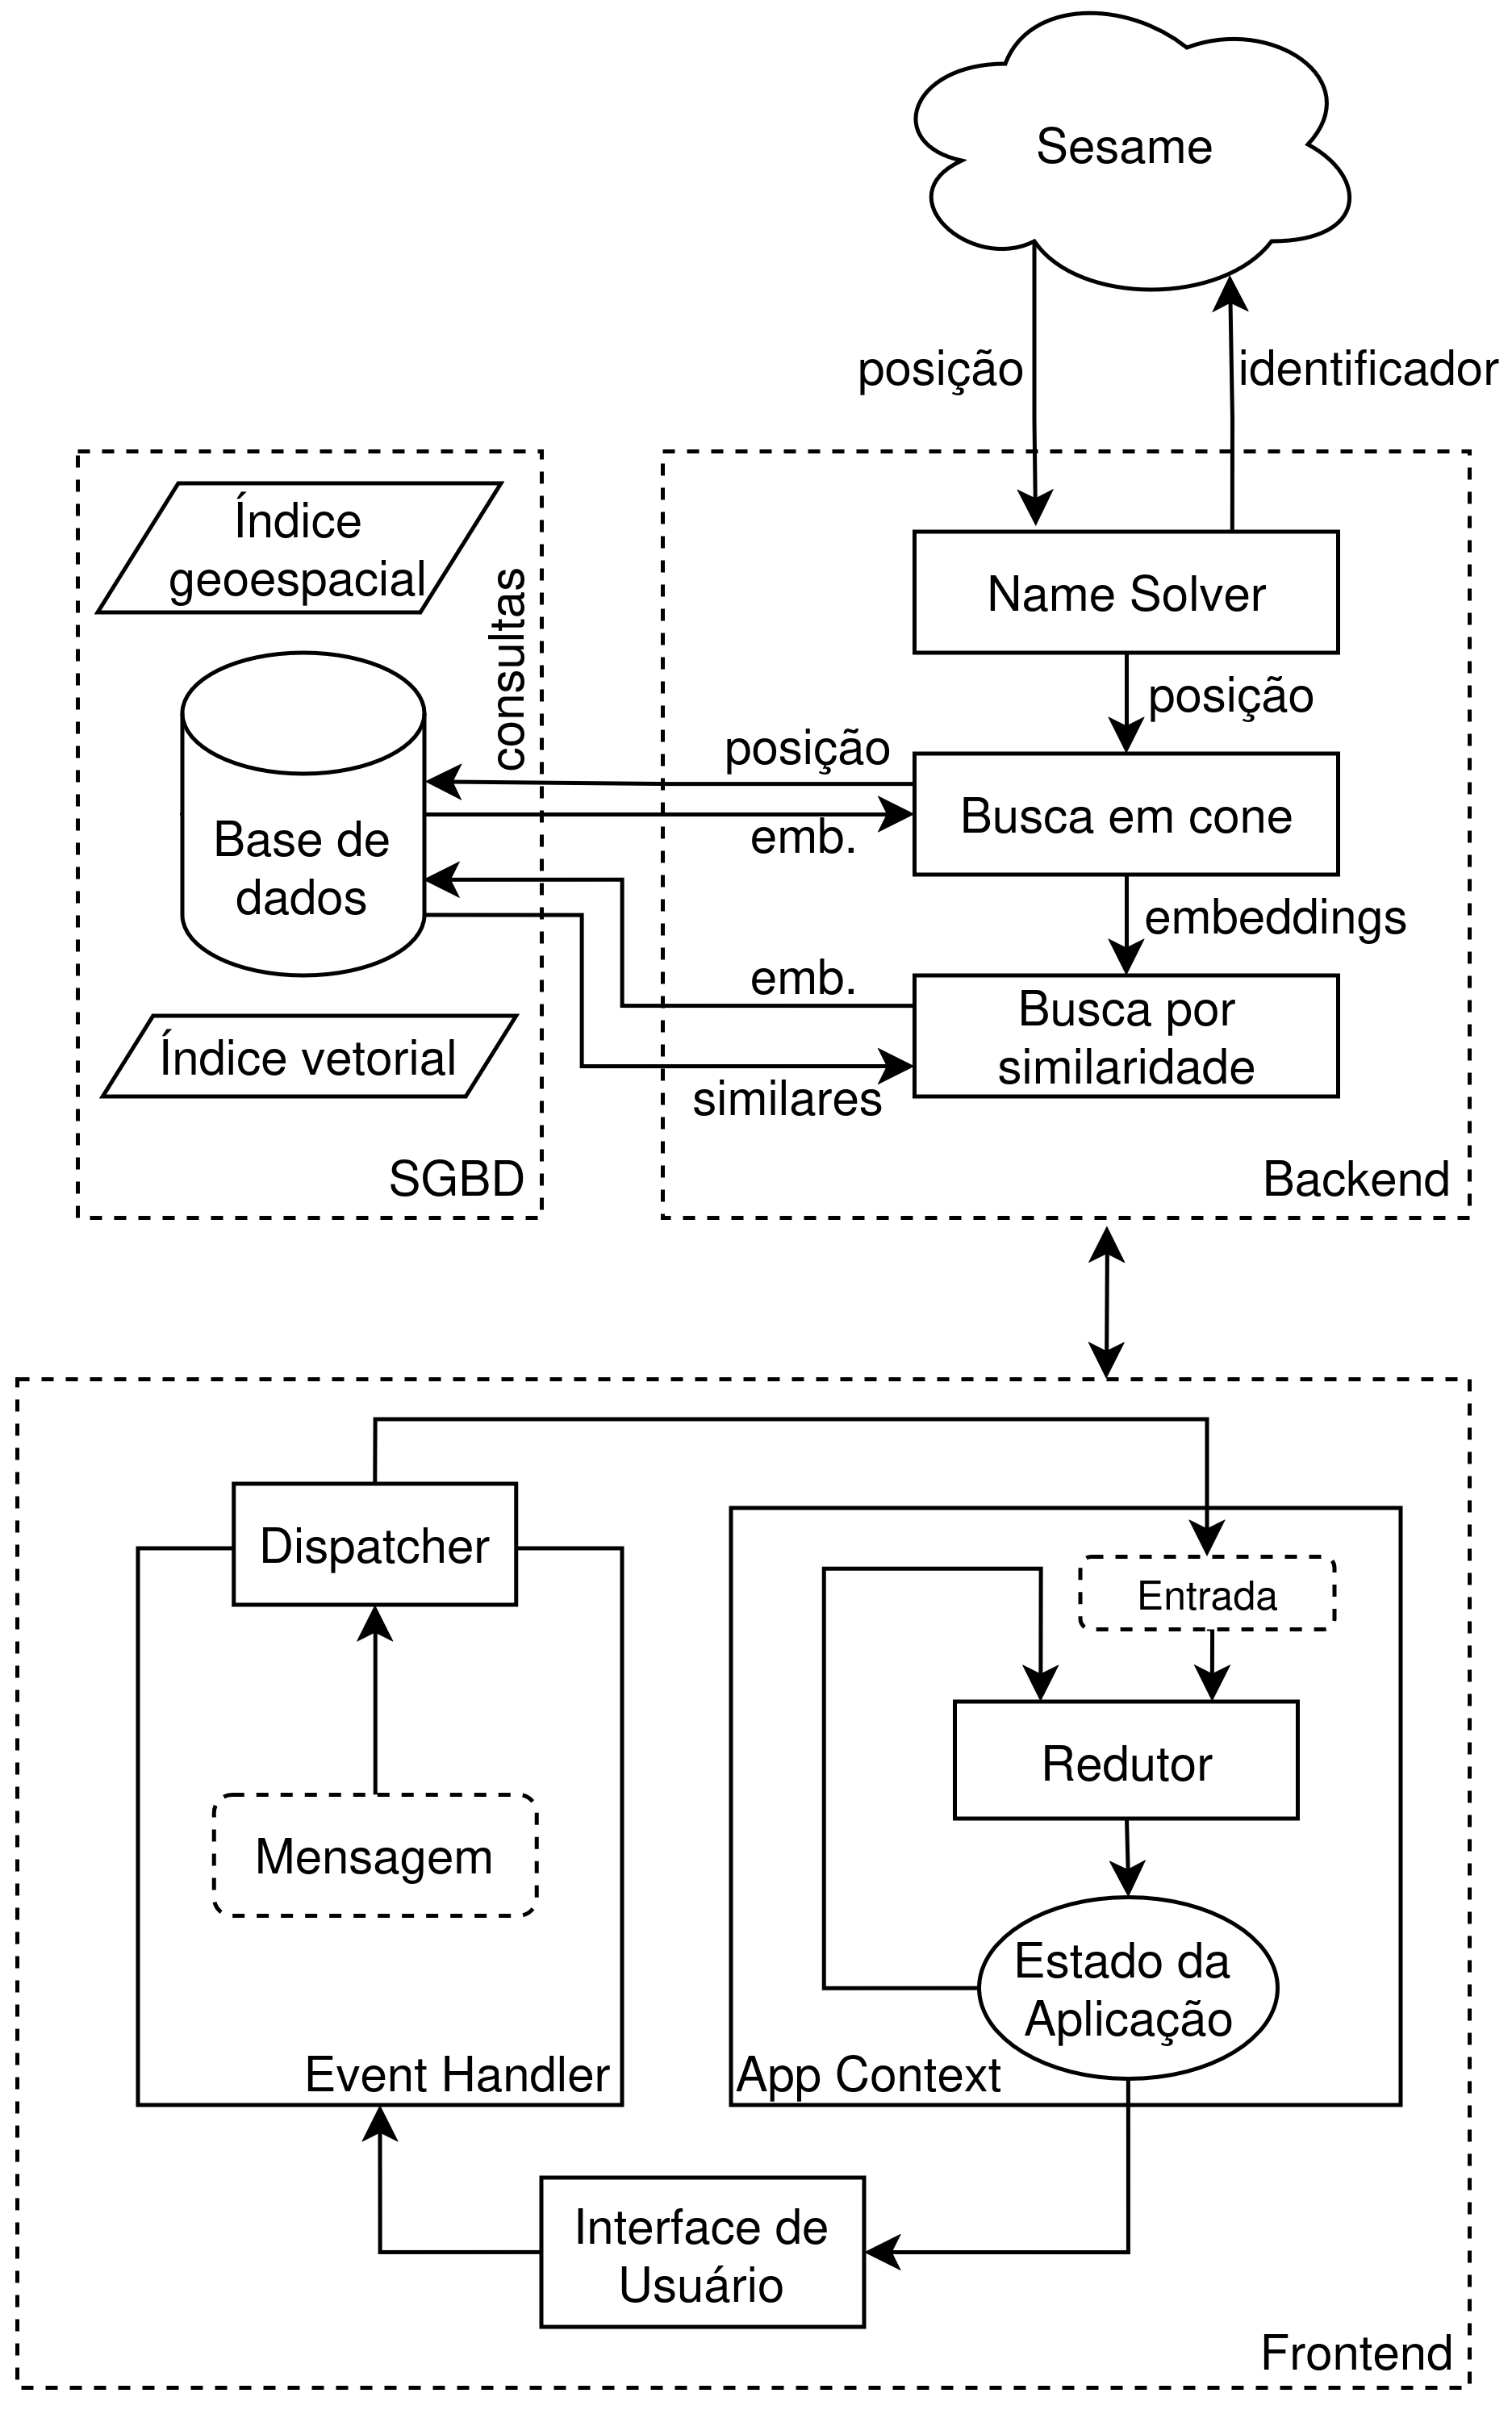
\includegraphics[width=0.75\linewidth]{figures/si.png}
\end{figure}


% \begin{figure}[!ht]
%   \centering
%   \caption{Fluxograma do desenvolvimento do sistema de informação}
%   \label{fig:flow-aquisicao}
%   \simpleflowdiagram{0.5}{
%     Base de Dados (Seção \ref{sec:si-db}),
%     Backend (Seção \ref{sec:si-backend}),
%     Frontend (Seção \ref{sec:si-frontend}),
%     Implantação (Seção \ref{sec:si-implantacao})
%   }
% \end{figure}



\subsection{Base de Dados}
\label{sec:si-db}

A base de dados desempenha um papel fundamental no sistema inteligente desenvolvido, pois ela tem a função de armazenar as representações visuais, geradas a partir do modelo do aprendizagem profunda (Seção \ref{sec:modelo}) e delimitadas pelo conjunto de inferência (Seção \ref{sec:aquisicao-inferencia}), com o propósito de viabilizar a busca rápida no céu por similaridade visual em uma grande área do céu. Esta funcionalidade foi especificada durante a concepção do projeto como o  requisito funcional de armazenamento e recuperação de representações visuais (Seção \ref{sec:req-db}). A seguir, são discutidas as tecnologias  (Seção \ref{sec:si-tecnologias}), o modelo de dados (Seção \ref{sec:si-datamodel}) e as otimizações (Seções \ref{sec:si-coords-index} e \ref{sec:si-vec-index}) utilizadas do desenvolvimento da base de dados.

% No Sistema Inteligente proposto, a base de dados tem a função de armazenar as representações visuais, geradas a partir do modelo do aprendizagem profunda (Seção \ref{sec:modelo}) e delimitadas pelo conjunto de inferência (Seção \ref{sec:aquisicao-inferencia}), com o propósito de viabilizar a busca rápida no céu por similaridade visual em uma grande área do céu.



\subsubsection{Tecnologias Utilizadas}
\label{sec:si-tecnologias}

Uma parte fundamental no projeto de uma base de dados é a escolha do Sistema Gerenciador de Banco de Dados (SGBD), essa escolha está fortemente relacionada com o tipo de dado a ser armazenado e os tipos de buscas a serem realizadas. Nesse sentido, para atender os requisitos da aplicação desenvolvida, as especificações do SGBD são listadas a seguir.

\begin{itemize}
  \item \textbf{Armazenamento de vetores:} as características visuais extraídas pelo modelo de aprendizagem profunda (Seção \ref{sec:modelo}) são representadas na forma de vetores. Logo, é essencial que o SGBD  consiga manusear esse tipo de dado;
  \item \textbf{Busca eficiente de vetores:} a recuperação de objetos similares é a busca por obejtos com menor distância do vetor de referêcia. Nesse sentido, o SGBD precisa realizar operações com distância de vetores além de ter um mecanismo de indexação que otimize a busca por distância;
  \item \textbf{Busca por posição:} além das representações visuais, a base de dados deve armazenar metadados dos objetos, como a posição. A busca por posição é fundamental para integrar o sistema como outros serviços web astronômicos, como Sesame, Simbad e Vizier, pois ela permite correlacionar informações de um mesmo objeto proveniente de fontes diferentes.
\end{itemize}

Com base nas especificações apresentadas e levando em consideração as tecnologias do estado-da-arte para a tarefa desenvolvida \cite{pan2024}, o PostgreSQL\footnote{\url{https://postgresql.org}} foi ecolhido como SGDB, pois sua flexibilidade e extensibilidade permitem as funcionalidades de busca por posição e vetorial, discutidas nas Seções \ref{sec:si-coords-index} e \ref{sec:si-vec-index}, respectivamente.


\subsubsection{Modelo de Dados}
\label{sec:si-datamodel}

A definição de um modelo de dados eficiente é fundamental para a integração das diversas partes do sistema. A Fig. \ref{fig:db} mostra o diagrama entidade-relacionamento da base de dados projetada para o armazenamento e a recuperação dos objetos por similaridade visual.

\begin{figure}[!ht]
  \centering
  \caption{Diagrama entidade-relacionamento da base de dados}
  \label{fig:db}
  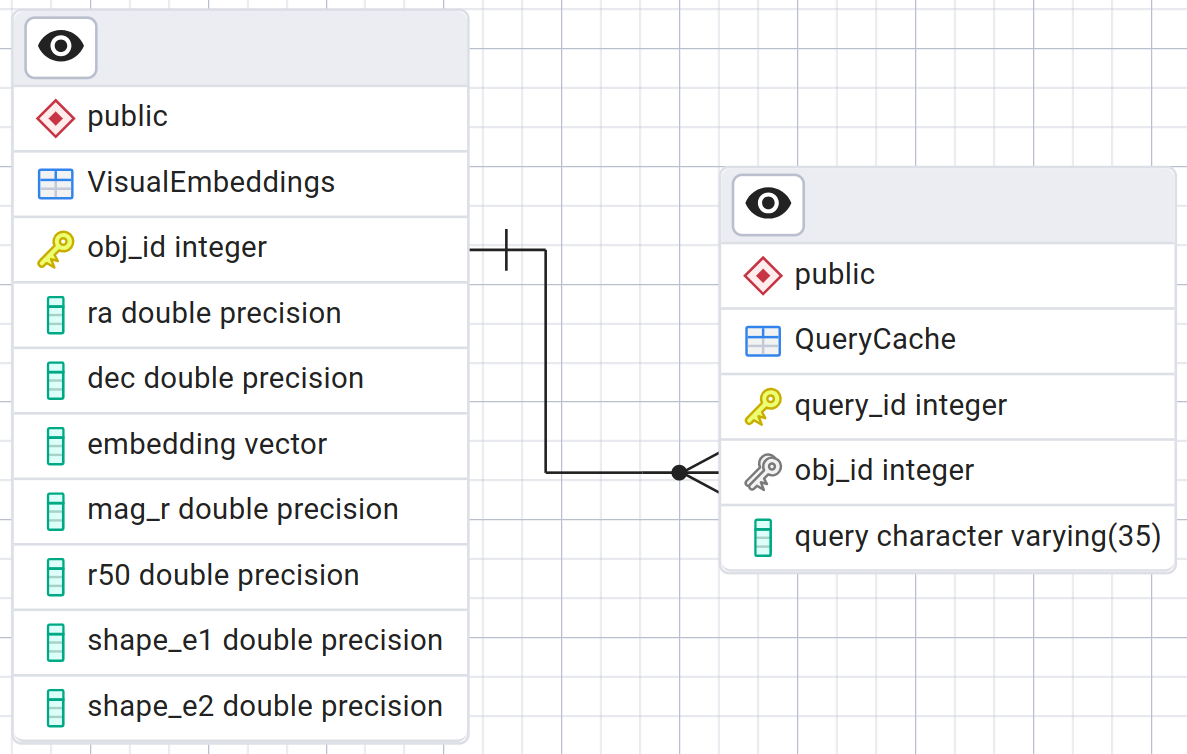
\includegraphics[width=\linewidth]{figures/database.png}
  \legend{O diagrama entidade-relacionamo mostra duas tabelas: \texttt{VisualEmbeddings} (esquerda) e \texttt{QueryCache} (direita). A primeira armazena as representações visuais e algumas propriedades físicas de todas as galáxias do conjunto de inferência (Seção \ref{sec:aquisicao-inferencia}). Já a segunda é um cache que associa um termo de busca à chave primária da tabela anterior, tendo a função de evitar requisição ao sistema Sesame e a correlação por coordenadas.}
\end{figure}


As Tabelas \ref{tab:VisualEmbeddings} e \ref{tab:QueryCache} informam o tipo de dado e uma breve descrição de cada coluna das tabelas mostradas na Fig. \ref{fig:db}.

A indexação de colunas é um mecanismo fundamental de otimização de consultas em bases de dados relacionais, representando os dados por uma estrutura de dados auxiliar, projetada para garantir mais desempenho em tipos específicos de problemas. Na sequência, são mostradas as técnicas de indexação para as colunas \texttt{ra} e \texttt{dec} (Seção \ref{sec:si-coords-index}) e para a coluna \texttt{embedding} (Seção \ref{sec:si-vec-index}).

\begin{table}[!ht]
  \centering
  \caption{Descrição da tabela VisualEmbeddings}
  \label{tab:VisualEmbeddings}
  \begin{tabular}{rlp{.6\linewidth}}
    \toprule
    Coluna    & Tipo           & Descrição                                                                     \\
    \midrule
    obj\_id   & inteiro        & Chave primária do objeto                                                      \\
    ra        & precisão dupla & Ascenção Reta do obejeto (Seção \ref{sec:sistema-coordenadas})                \\
    dec       & precisão dupla & Declinação do obejeto (Seção \ref{sec:sistema-coordenadas})                   \\
    embedding & vetor          & Vetor de representações visuais                                               \\
    mag\_r    & precisão dupla & Magnitude do objeto (Seção \ref{sec:magnitude})                               \\
    shape\_e1 & precisão dupla & Componente real da elipticidade complexa (Seção \ref{sec:elipticidade})       \\
    shape\_e2 & precisão dupla & Componente imaginária da elipticidade complexa (Seção \ref{sec:elipticidade}) \\
    % fov       & precisão dupla & Campo de visão angular ideal para o objeto, em arcsec (Seção \ref{sec:aquisicao-fov})     \\
    \bottomrule
  \end{tabular}
\end{table}


\begin{table}[!ht]
  \centering
  \caption{Descrição da tabela QueryCache}
  \label{tab:QueryCache}
  \begin{tabular}{rlp{.6\linewidth}}
    \toprule
    Coluna    & Tipo    & Descrição                                                                                                     \\
    \midrule
    query\_id & inteiro & Chave primária                                                                                                \\
    obj\_id   & inteiro & Chave estrangeira referenciando a coluna obj\_id da tabela VisualEmbeddings (Tab. \ref{tab:VisualEmbeddings}) \\
    query     & string  & Termo de busca utilzado para fazer a consulta                                                                 \\
    \bottomrule
  \end{tabular}
\end{table}



\subsubsection{Armazenamento e Indexação das Coordenadas}
\label{sec:si-coords-index}

A indexação das coordenadas, definidas pelas colunas \texttt{ra} e \texttt{dec}, utiliza o mecanismo Quad Tree Cube\footnote{\url{https://github.com/segasai/q3c}} (Q3C; \citealp{q3c}), que é uma técnica utilizada na astronomia para otimizar o armazenamento e a recuperação de dados espaciais em bancos de dados de grandes levantamentos astronômicos. Esse mecanismo foi desenvolvido para lidar com a quantidade massiva de dados gerada por observatórios modernos, que capturam informações sobre bilhões de objetos celestes, incluindo sua posição, brilho e outras características. A principal função do Q3C é permitir consultas eficientes em catálogos astronômicos, possibilitando a localização rápida de objetos com base em suas coordenadas celestes (Seção \ref{sec:sistema-coordenadas}).

O Q3C utiliza uma estrutura baseada em árvore quad (ou quadtree) projetada para dividir iterativamente a superfície da esfera celeste (Seção \ref{sec:sistema-coordenadas}) em regiões menores, como mostra a Fig. \ref{fig:q3c}. Cada região é identificada por um índice (chamado IPIX), o que permite armazenar e acessar informações de localização de forma hierárquica. No Q3C, a superfície esférica é projetada em um cubo e subdividida em quadrantes, o que facilita a representação de posições celestes e otimiza a indexação espacial. Essa estrutura de dados permite que consultas espaciais, como encontrar todos os objetos dentro de um certo raio de um ponto específico, sejam executadas com alta eficiência, reduzindo a necessidade de examinar todas as entradas do catálogo.

\begin{figure}[!ht]
  \centering
  \caption{Segmentação da esfera celeste pelo Q3C}
  \label{fig:q3c}
  \begin{overpic}[width=.32\linewidth]{figures/q3c_1.png}
    \put (0,90) {(a)}
  \end{overpic}\hfill
  \begin{overpic}[width=.32\linewidth]{figures/q3c_2.png}
    \put (0,90) {(b)}
  \end{overpic}\hfill
  \begin{overpic}[width=.32\linewidth]{figures/q3c_3.png}
    \put (0,90) {(c)}
  \end{overpic}
  \legend{Nos painéis (a) e (b), são mostradas segmentações da esfera celeste (Seção \ref{sec:sistema-coordenadas}) pelo Q3C para duas quantidades de bits distintas. Já o painel (c) mostra um exemplo de busca usando o Q3C. Fonte: Compilação das Figs. 1 e 2 de \citeonline{q3c}.}
\end{figure}

A implementação do Q3C aproveita funções de hashing para transformar as coordenadas esféricas em valores que podem ser facilmente indexados. Esse processo de hash mapeia coordenadas (RA, DEC) para uma representação numérica, permitindo uma indexação que é eficiente tanto para operações de busca por proximidade quanto para consultas de intervalo. As consultas são formuladas de maneira que a hierarquia de quadrantes seja explorada, de modo que apenas uma fração dos dados seja analisada para atender à consulta. Além disso, o Q3C pode realizar operações de cruzamento de catálogos, comparando dados de diferentes levantamentos com rapidez.


\subsubsection{Armazenamento e Indexação dos Vetores}
\label{sec:si-vec-index}

Embora o PostgreSQL seja tradicionalmente um banco de dados relacional, sua flexibilidade e extensibilidade permitem a implementação de funcionalidades tipicamente associadas a bancos de dados vetoriais \cite{taipalus2024}, como o armazenamento e a busca eficiente de vetores. Isso é alcançado por meio de extensões, como o pgvector\footnote{\url{https://github.com/pgvector/pgvector}}, que integram capacidades vetoriais ao PostgreSQL. Com essa abordagem, é possível armazenar vetores diretamente em tabelas relacionais e realizar consultas por similaridade, transformando o PostgreSQL em uma solução híbrida que combina recursos relacionais e vetoriais.

O mecanismo de indexação de vetores no pgvector é projetado para otimizar a indexação e busca de embeddings de alta dimensionalidade, especialmente aqueles gerados por modelos de aprendizagem profunda. Tais representações são amplamente utilizadas em aplicações como recuperação de informação, recomendação e classificação de dados, onde é necessário medir similaridade entre itens com base em seus embeddings. O pgvector oferece suporte nativo para armazenar e indexar esses vetores no PostgreSQL, tornando viável a realização de buscas eficientes mesmo em bancos de dados com grandes volumes de dados vetoriais.

O pgvector utiliza o HNSW, uma estrutura de grafos, chamada Hierarchical Navigable Small World Graph (HNSW; \citealp{hnsw}), que facilita a busca aproximada por similaridade. O HNSW é baseado em uma hierarquia de grafos navegáveis, onde cada nó representa um vetor, e conexões entre nós são criadas com base na similaridade vetorial. Esse grafo permite uma navegação eficiente, utilizando uma busca aproximada que, apesar de não garantir a precisão absoluta, oferece um bom equilíbrio entre desempenho e precisão. O HNSW é particularmente eficaz em cenários com alta dimensionalidade, pois reduz o número de cálculos de similaridade necessários para encontrar o vetor mais próximo, sendo capaz de realizar buscas sublineares em grandes volumes de dados. Em termos de aplicação prática, esse método torna viável a busca por similaridade em bancos de dados com milhões de embeddings, permitindo um tempo de resposta mais rápido.



\subsection{Backend}
\label{sec:si-backend}

O backend refere-se à camada responsável pelo processamento lógico, manipulação de dados e comunicação com bancos de dados e serviços externos. Ele opera nos servidores e é invisível ao usuário final, funcionando como a infraestrutura que sustenta e executa as operações solicitadas pelo frontend. O backend normalmente utiliza frameworks e ferramentas para gerenciar APIs, autenticação, controle de acesso e persistência de dados. Sua principal função é garantir que as informações sejam processadas de forma segura, eficiente e escalável, permitindo que a aplicação ofereça funcionalidades dinâmicas aos usuários.


\subsubsection{Tecnologias Utilizadas}
\label{sec:si-back-tech}

O desenvolvimento do backend requer a utilização de tecnologias que garantam desempenho, escalabilidade e flexibilidade. Nesse contexto, a biblioteca Blacksheep\footnote{\url{https://www.neoteroi.dev/blacksheep}}, implementada em Python, oferece uma solução moderna para construir APIs robustas e eficientes. Trata-se de um framework assíncrono que utiliza o modelo de programação baseado em corrotinas do Python, permitindo lidar de maneira eficiente com operações de entrada e saída (E/S) intensivas, como consultas a bancos de dados de grande escala.

A Blacksheep é projetada sobre o motor de eventos do módulo asyncio, proporcionando suporte nativo para o desenvolvimento de APIs RESTful de alta performance. Sua abordagem assíncrona é vantajosa para sistemas que requerem comunicação frequente com bancos de dados, como é o caso deste sistema de recuperação de imagens astronômicas. Além disso, a biblioteca adota um design simples e modular, permitindo personalizar funcionalidades conforme necessário.

Foram utilizados os middlewares e roteamento eficiente da biblioteca Blacksheep, possibilitando a construção de uma API organizada e segura. A biblioteca também integra-se facilmente com o SQLAlchemy, essencial em aplicações astronômicas, que frequentemente demandam operações complexas de busca e agregação de dados.

% Adicionalmente, a Blacksheep oferece suporte a recursos como validação de dados, serialização e uso de controladores baseados em classes, promovendo uma estrutura clara e sustentável para o código. A compatibilidade com tecnologias modernas, como OpenAPI e JSON Schema, facilita a documentação automática da API, melhorando a interoperabilidade e o desenvolvimento colaborativo. Essas vantagens tornam a Blacksheep uma escolha ideal para implementar o backend de um sistema que requer alta responsividade, modularidade e suporte a consultas complexas, como a recuperação de imagens por similaridade visual em astronomia.




\subsubsection{Integrações}
\label{sec:si-back-arch}

O backend é composto por uma API RESTful responsável por implementar a lógica de consulta por similariade e permitir o acesso aos dados pelo frontend. Pensando em aumentar a flexibilidade e a experiência de usuário, o sistema permite que a busca seja feito pelo nome oficial da galáxia, apelido ou coordenada. Para garantir essa funcionalidade, é necessária uma interação com o webserviço astronômico \emph{Sesame Name Solver}\footnote{\url{https://cds.unistra.fr/cgi-bin/Sesame}}, que é utilizado para resolver o termo de busca enviado pelo usuário, convertendo-o em posição angular da galáxia (RA e Dec).

% Buscas por posição e por similaridade são feitas pelo backend para




% \begin{figure}[!ht]
%   \centering
%   \caption{Diagrama da arquitetura do backend}
%   \label{fig:backend}
%   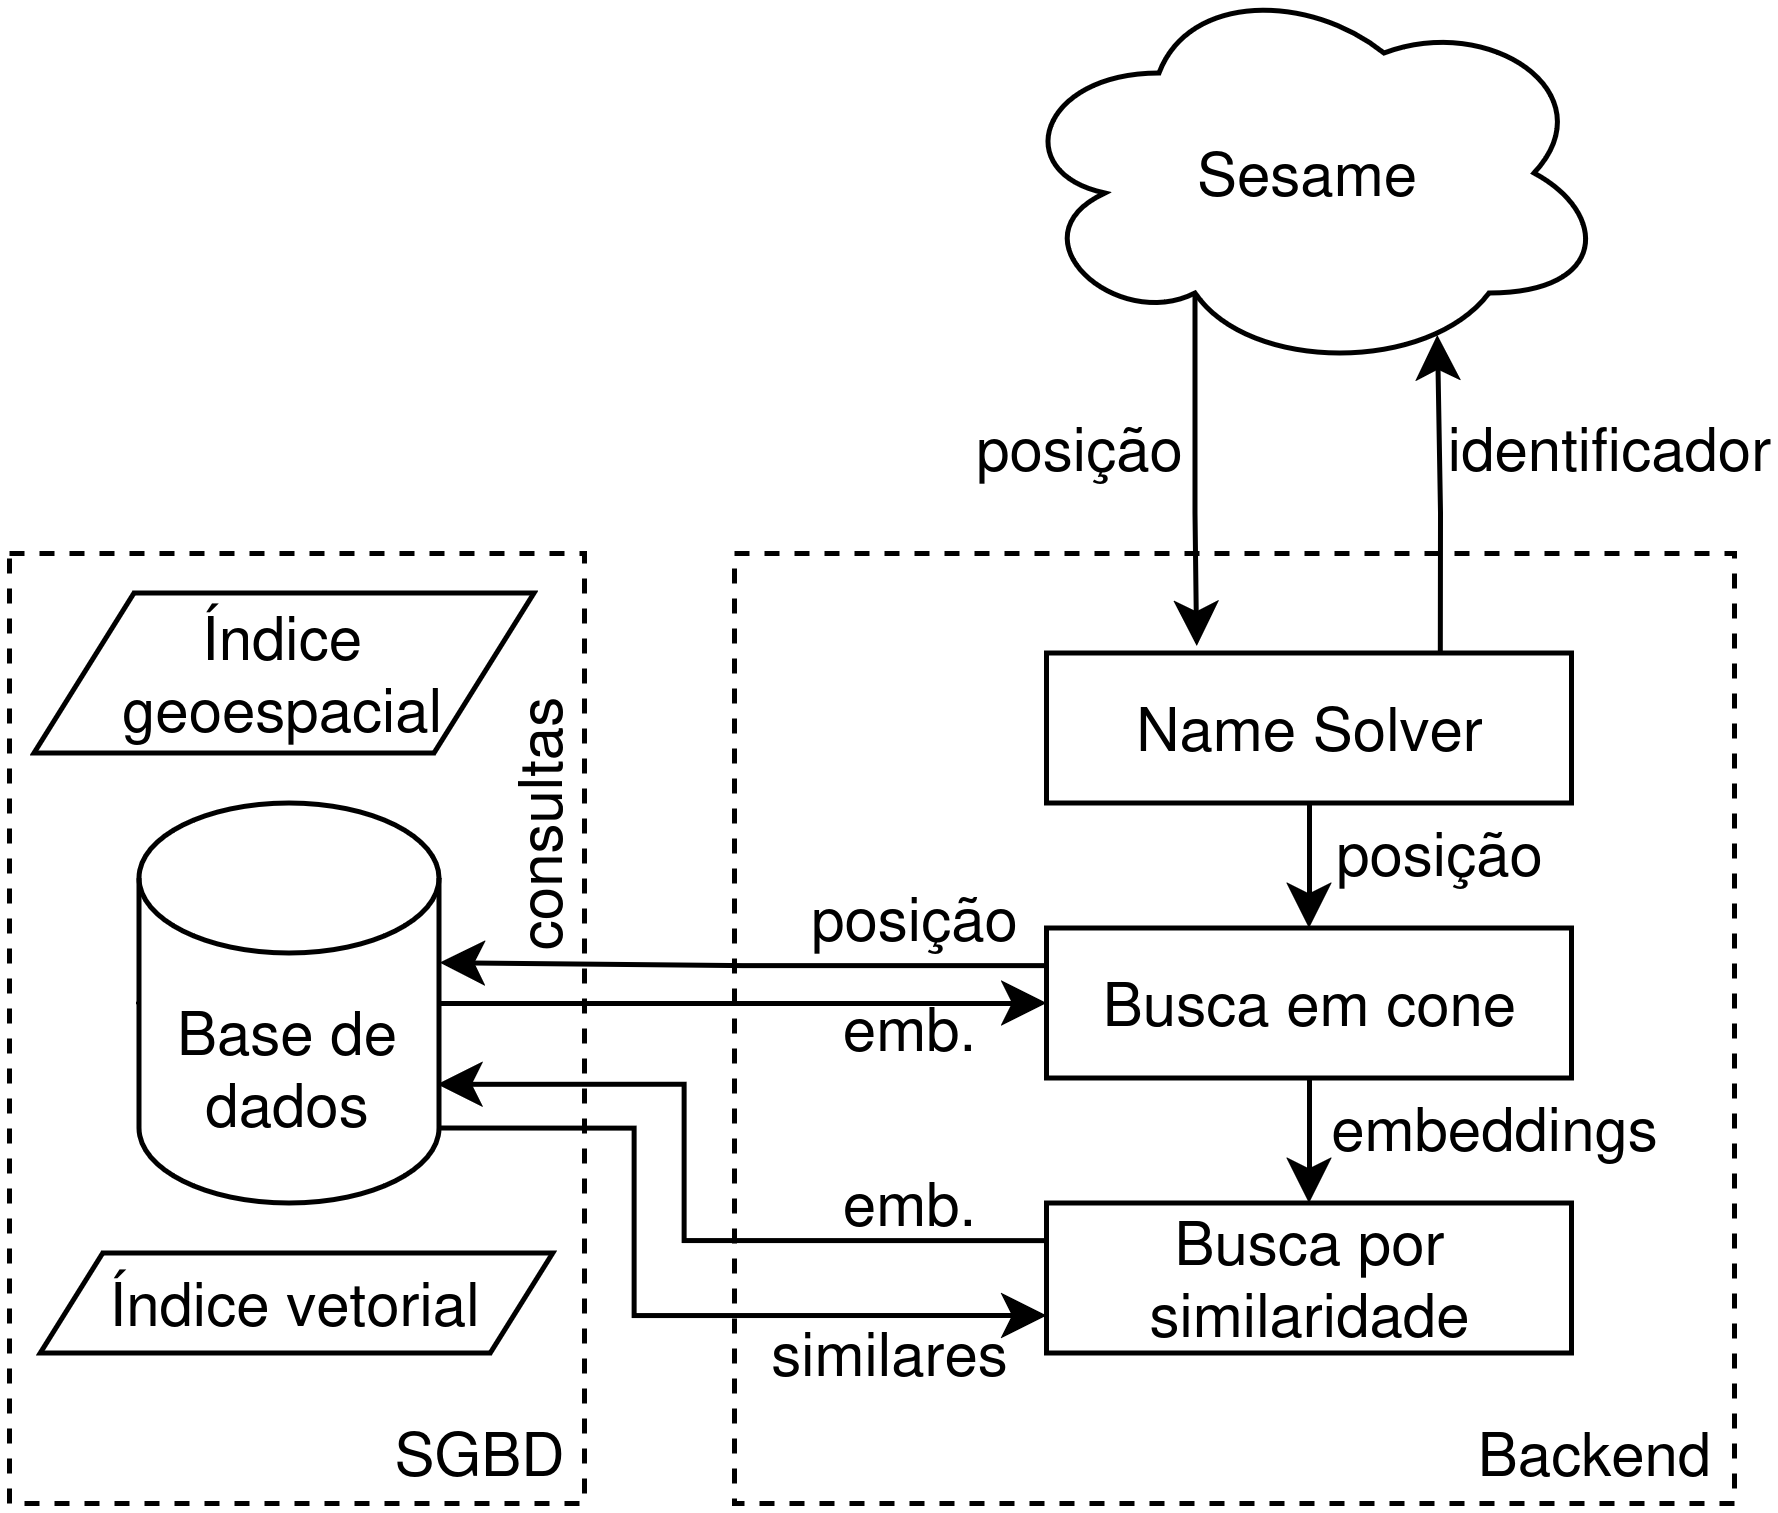
\includegraphics[width=0.8\linewidth]{figures/backend.png}
% \end{figure}




\subsubsection{Procedimento de Busca no Backend}
\label{sec:si-bacak-busca}

A Fig. \ref{fig:seq-back} mostra o diagrama de sequência do procedimento de busca por similaridade visual do ponto de vista do backend. Nela é mostrada as três etapas da busca: a resolução do nome do objeto, transformando-o em coordenadas; a busca por posição no banco de dados para encontrar os embeddings da galáxia buscada e, por fim, a busca por similaridade.

\begin{figure}[!ht]
  \centering
  \caption{Diagrama de sequência da busca no backend}
  \label{fig:seq-back}
  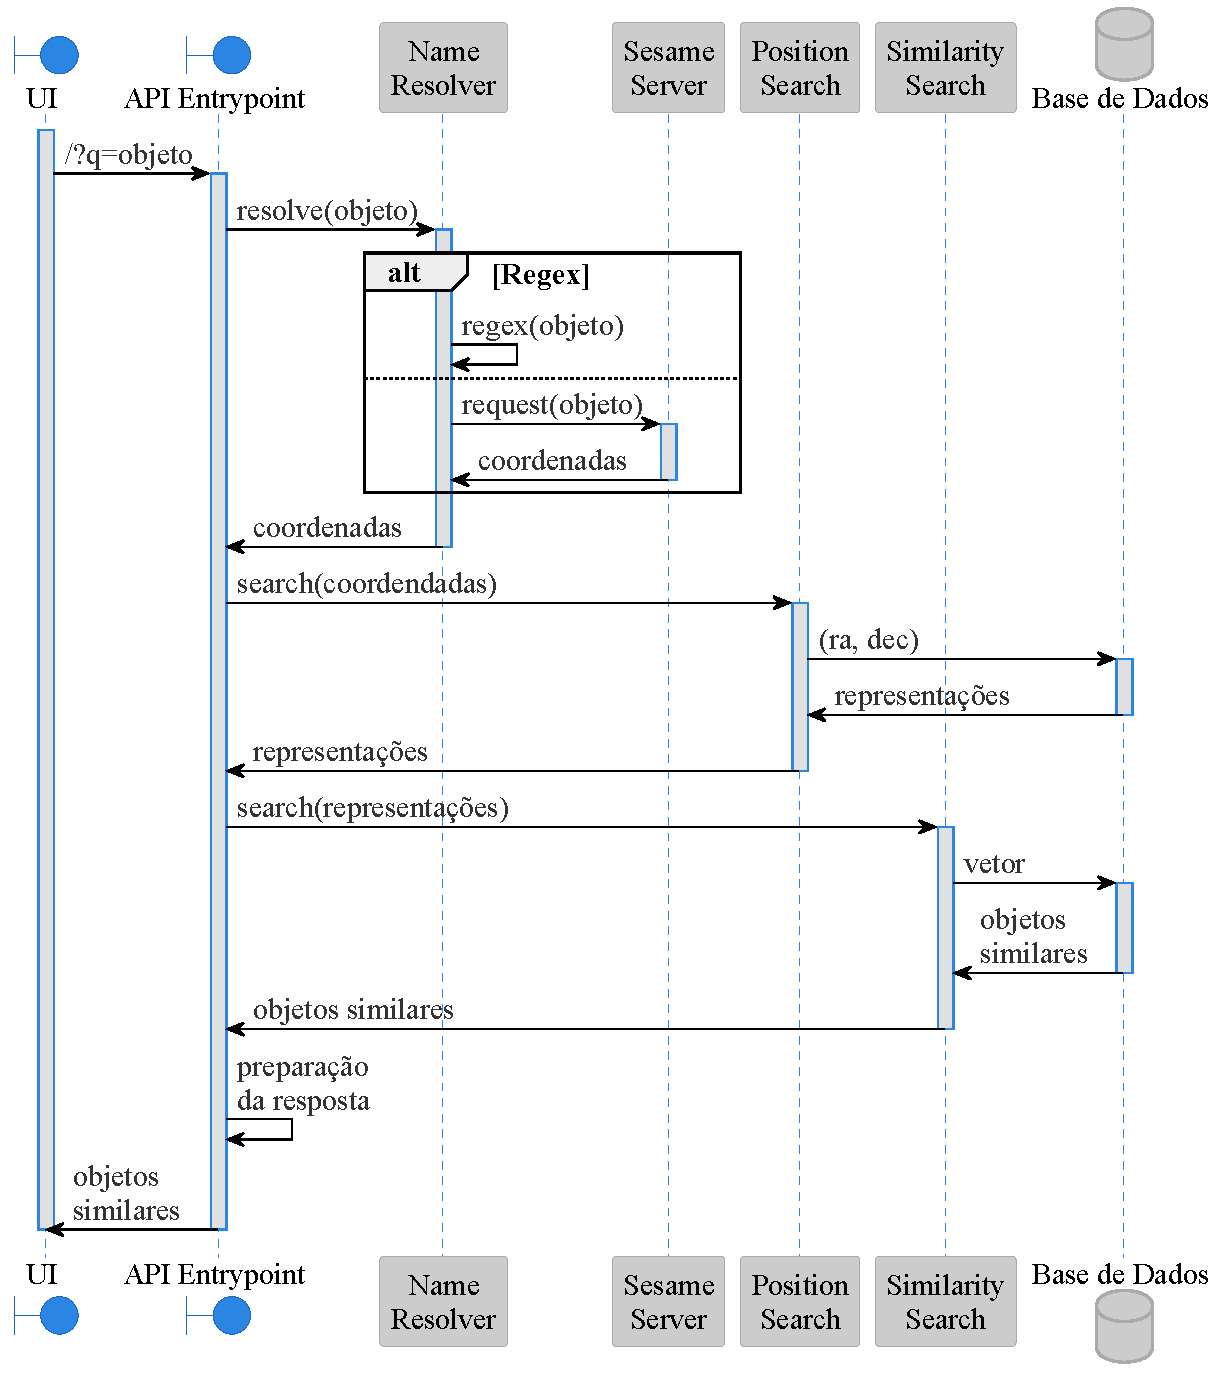
\includegraphics[width=\linewidth]{diagrams/plots/sequence_back.pdf}
  \legend{Primeiramente, o termo de busca é decodificado em coordenadas RA e Dec utilizando o webserviço Sesame. Em seguida, uma busca por posição é feita no banco de dados para obter as representações da galáxia busca. Por fim, é feita uma busca por similaridade para obter as galáxias similares.}
\end{figure}






\subsection{Frontend}
\label{sec:si-frontend}

O frontend refere-se à camada da aplicação interpretada diretamente pelo navegador responsável pela interface visual e interação direta com o usuário. Ele abrange a estrutura, o estilo e o comportamento das páginas ou telas que os usuários visualizam e utilizam. O frontend conecta-se ao back-end por meio de APIs, recebendo e enviando dados para apresentar informações dinâmicas e garantir uma experiência de uso interativa e responsiva.


\subsubsection{Tecnologias Utilizadas}
\label{sec:si-front-tech}

O frontend é a camada da aplicação que é executada no navegador. Ele foi desenvolvido em TypeScript\footnote{\url{https://typescriptlang.org}}, que é uma linguagem de programação de código aberto que expande o JavaScript ao adicionar suporte a tipagem estática e outras funcionalidades avançadas de desenvolvimento. O TypeScript é amplamente utilizado para melhorar a robustez e a escalabilidade do código, permitindo a detecção de erros em tempo de compilação e facilitando a manutenção de projetos complexos. As aplicações feitas nesta linguagem são transpiladas para JavaScript para serem interpretadas pelos navegadores.

O frontend foi desevolvido utilzando o Next.js\footnote{\url{https://nextjs.org}}, que é um framework de desenvolvimento web baseado na biblioteca React que permite a criação de aplicações modernas e escaláveis. A principal ferramenta usada é a geração estática (Static Site Generation, SSG), que permite compilar e distribuir o frontend como uma aplicação completamente independente do backend. Além disso, o Next.js fornece uma estrutura que simplifica o desenvolvimento ao incluir funcionalidades integradas, como roteamento automático baseado em arquivos, suporte a APIs serverless, otimização de desempenho e internacionalização.

A biblioteca React\footnote{\url{https://react.dev}} revolucionou a forma como interfaces de usuário (UI) são projetadas e construídas no desenvolvimento de aplicativos modernos. Baseada no conceito de componentes reutilizáveis, o React permite que desenvolvedores criem aplicações web e móveis de forma declarativa, eficiente e altamente escalável.


\subsubsection{Arquitetura}
\label{sec:si-front-arch}

Um dos principais diferenciais do React é sua abordagem declarativa para o desenvolvimento de UI. Em vez de manipular diretamente o Document Object Model (DOM), os desenvolvedores descrevem como a interface deve se comportar em diferentes estados, e o React cuida de atualizar o DOM de maneira eficiente. Essa abstração é possibilitada pelo Virtual DOM, uma representação leve do DOM real que permite ao React identificar e aplicar somente as alterações necessárias, minimizando a manipulação direta do DOM e melhorando o desempenho de aplicativos, especialmente em sistemas complexos com múltiplos estados dinâmicos.


\begin{figure}[!ht]
  \centering
  \caption{Arquitetura do gerenciamento de estado da interface de usuário}
  \label{fig:arch-front}
  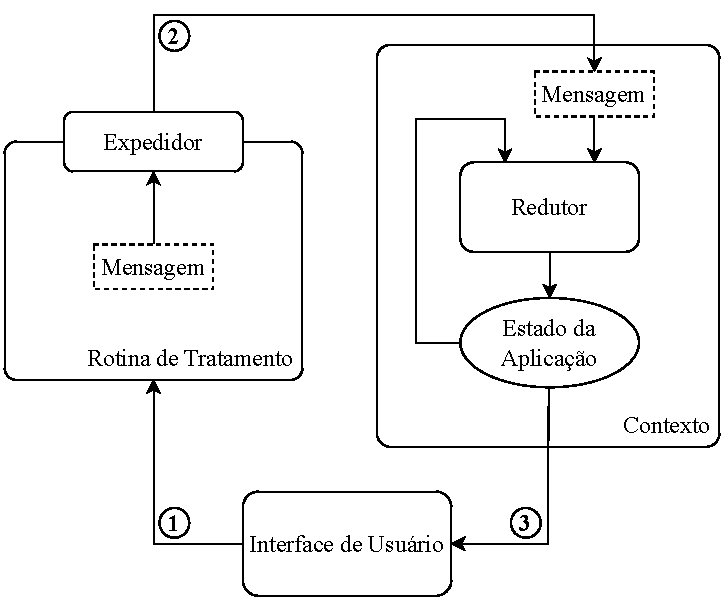
\includegraphics[width=0.8\linewidth]{figures/flow_front.pdf}
\end{figure}

Nessa abordagem declarativa, o gerenciamento de estado da aplicação é o mecanismo mais importante. Este mecanismo pode ser visto como uma máquina de estados finita \cite{formal-methods} que depende do estado atual e uma entrada para produzir o próximo estado, como a máquina \citeonline{mealy}. Este mecanismo é ilustrado no diagrama da Fig. \ref{fig:arch-front} e seus elementos são explicados a seguir.

\begin{enumerate}
  \item O usuário interage com a \emph{Interface do Usuário} (UI), causando um evento, que é enviado para a \emph{Rotina de Tratamento}. Este evento pode ser um clique do mouse, um pressionamento de tecla, uma seleção de arquivo e assim por diante.
  \item A \emph{Rotina de Tratamento} é a função responsável por processar o evento. Como o sistema é desenvolvido usando abordagem declarativa, ao invés de executar alterações diretas na UI, esta função prepara uma mensagem contendo todas as informações necessárias para mudar a aplicação para outro estado e passá-la para o \emph{Expedidor}, responsável por enviar a mensagem para o \emph{Redutor}.
  \item O \emph{Redutor} é a função, chamada pelo \emph{Contexto da Aplicação}, responsável por gerar o próximo estado da aplicação. Esta função recebe o estado atual e a mensagem do \emph{Expedidor} para criar um novo estado. A mutação no \emph{Estado da Aplicação} dispara a atualização da UI, realizada pela biblioteca React. O \emph{Redutor} pode ser visto como a função de transição da Máquina Mealy.
\end{enumerate}


Além disso, a arquitetura baseada em componentes do React é outro ponto crucial para seu sucesso. Aplicações são divididas em partes menores e independentes, chamadas componentes, que encapsulam lógica, estilo e estrutura de forma modular. Esses componentes podem ser reutilizados em diferentes partes de um aplicativo ou até mesmo em projetos distintos, promovendo consistência no design e eficiência no desenvolvimento. Além disso, a reutilização de componentes reduz o tempo necessário para implementar novas funcionalidades e simplifica a manutenção do código, uma característica essencial para projetos modernos, que frequentemente envolvem equipes de desenvolvimento distribuídas e de grande escala.


\subsubsection{Procedimento de Busca no Frontend}
\label{sec:si-front-busca}

A Fig. \ref{fig:seq-front} mostra o diagrama de sequência do procedimento de busca por similaridade visual do ponto de vista do frontend.

\begin{figure}[!ht]
  \centering
  \caption{Diagrama de sequência da busca no frontend}
  \label{fig:seq-front}
  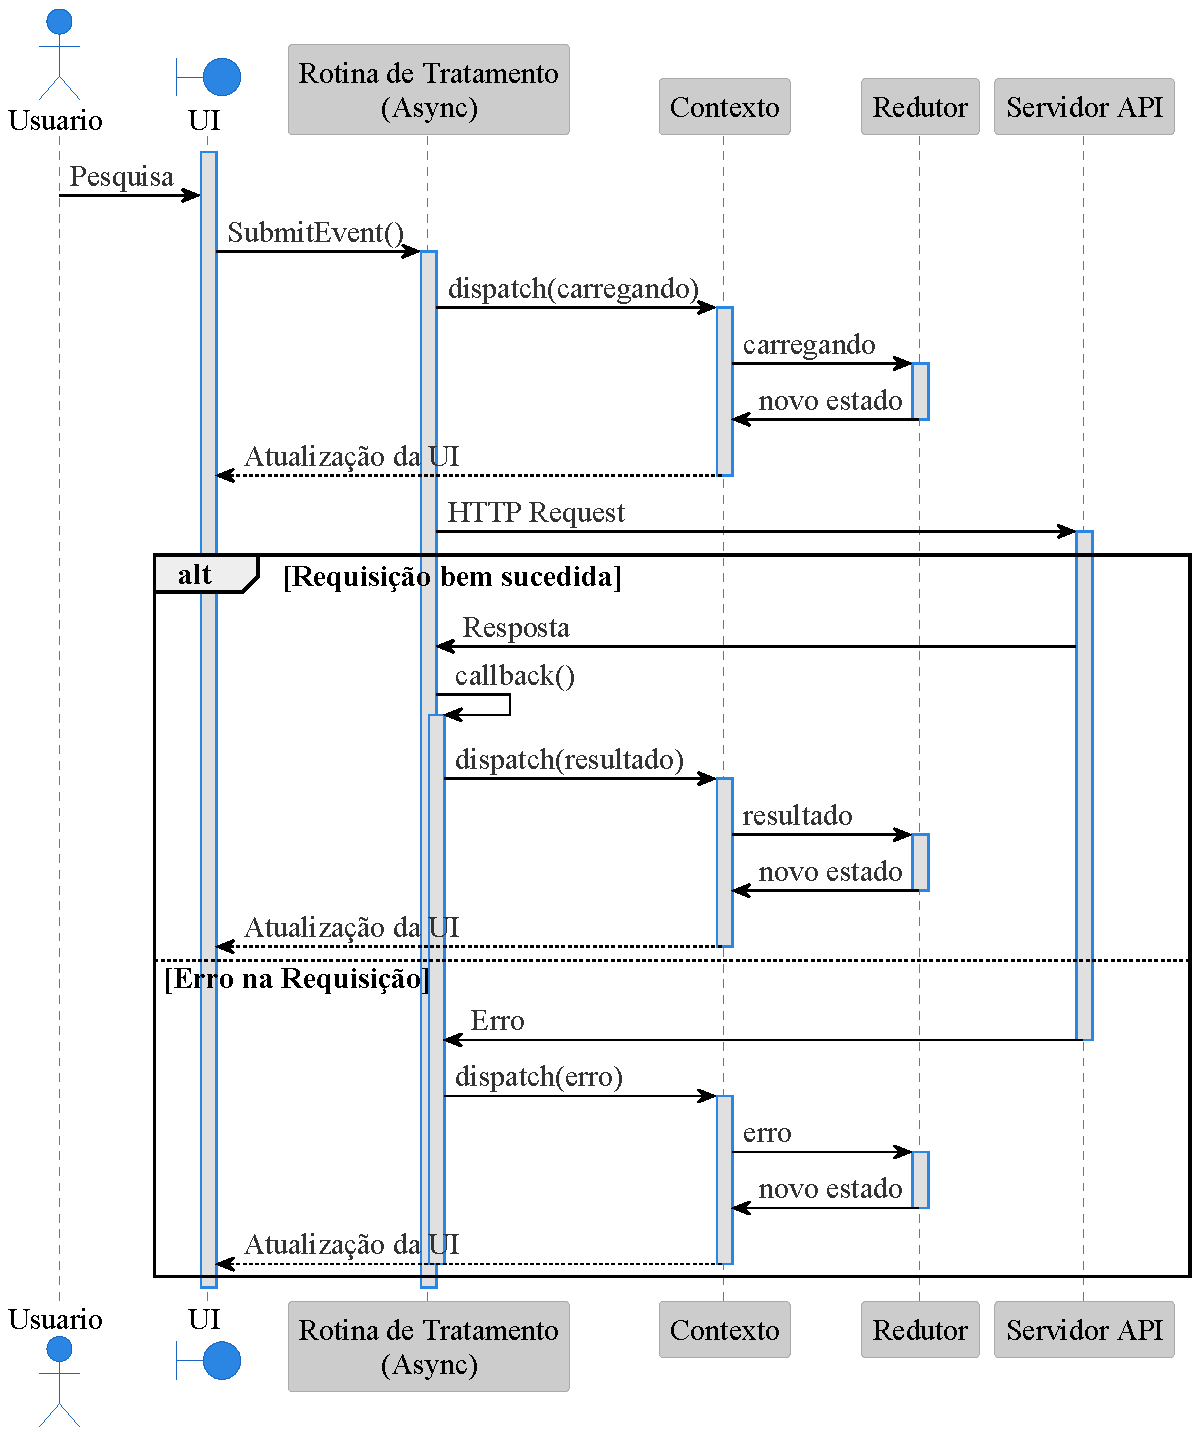
\includegraphics[width=\linewidth]{diagrams/plots/sequence_front.pdf}
  \legend{Ao interagir com a barra de pesquisa, o usuário engatilha um evento, que é interceptado pelo motor de eventos do navegador, que inicializa a rotina de tratamento registrada para o evento. Esta função despacha uma mensagem, ao contexto da aplicação, para mudar o estado da UI para ``carregando'' e, em seguida, faz uma requisição HTTP ao servidor. Ao receber a resposta da API, a função callback é responsável por despachar uma mensagem com os resultados ou com erro, causando uma nova atualização da UI.}
\end{figure}



\subsection{Implementação e Implantação}
\label{sec:si-implantacao}

Nesta seção, são abordadas as técnicas de desenvolvimento e implantação utilizadas para a disponibilização do sistema de informação desenvolvido como uma aplicação web.


\subsubsection{Sistema de Controle de Versão}
\label{sec:si-devops}

O uso combinado do sistema de controle de versão Git e da plataforma GitHub\footnote{\url{https://github.com}} no desenvolvimento de um sistema inteligente para busca de imagens similares em astronomia oferece uma série de vantagens que otimizam a colaboração, a gestão do código e a automação de processos. O Git\footnote{\url{https://git.org}}, sendo um sistema distribuído, permite que os desenvolvedores rastreiem todas as alterações feitas no código-fonte de forma detalhada, possibilitando reverter modificações indesejadas e garantir a integridade do desenvolvimento. Sua estrutura descentralizada assegura que cada colaborador mantenha uma cópia completa do repositório, aumentando a segurança e a resiliência contra falhas.

A integração com o GitHub amplia essas capacidades, oferecendo uma interface intuitiva e funcionalidades adicionais que promovem o trabalho em equipe. A plataforma facilita a criação de ramificações (branches) para desenvolvimento paralelo, revisão de código por meio de pull requests e resolução de conflitos de forma transparente. Tais recursos são fundamentais em projetos de sistemas inteligentes, onde equipes frequentemente trabalham em componentes diferentes, como algoritmos de similaridade, infraestrutura de backend e interfaces gráficas.

Além disso, o GitHub fornece ferramentas de integração contínua (CI) e entrega contínua (CD), permitindo a execução automática de testes, validações e implantações a cada mudança no código. Isso reduz significativamente o risco de erros e acelera o ciclo de desenvolvimento, o que é crucial em projetos que lidam com grandes volumes de dados astronômicos. Recursos como issues e projetos também facilitam o gerenciamento de tarefas, promovendo organização e transparência.

% Outra vantagem é a documentação centralizada e o compartilhamento de conhecimento. Por meio de wikis e repositórios públicos ou privados, o GitHub permite armazenar e compartilhar informações detalhadas sobre o sistema, como arquitetura, uso de algoritmos e fluxo de dados. Isso é especialmente útil em contextos acadêmicos, incentivando a colaboração entre equipes e a disseminação de resultados científicos. Assim, o uso do Git e do GitHub contribui de maneira significativa para a eficiência, organização e confiabilidade do desenvolvimento de sistemas inteligentes em astronomia.


% \subsubsection{DevOps}
% \label{sec:si-devops}

% \begin{figure}[!ht]
%   \centering
%   \caption{Integração contínua}
%   \label{fig:ci-cd}
%   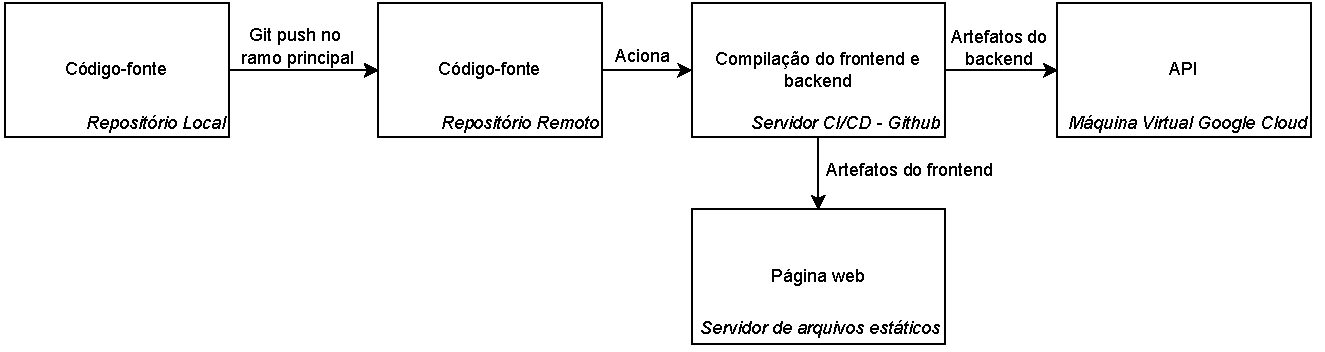
\includegraphics[width=\linewidth]{figures/ci-cd.pdf}
% \end{figure}

% A uso de práticas DevOps e pipelines de integração contínua e entrega contínua (CI/CD) com o GitHub no desenvolvimento do sistema de informação de um sistema inteligente para busca de imagens similares em astronomia oferece vantagens significativas em termos de automação, colaboração e qualidade do software. Este procedimento promove uma forma de integração entre desenvolvimento e operações, facilitando o gerenciamento eficiente de infraestrutura e aplicações.

% Como mostra a Fig. \ref{fig:ci-cd}, as pipelines de CI/CD foram configuradas no GitHub para serem acionadas quando ocorrer alguma atualização no ramo principal, automatizando a execução de validação de código e implantação de novas versões do sistema. A pipeline compila o frontend e o backend, que são despachados automanticamente para servidores distintos. Os arquivos estáticos do frontend (HTML, CSS, JS, imagens) são enviados ao serviço de hospedagem de arquivos estáticos e páginas web do próprio Github. Já o backend é enviado à uma máquina virtual do Google Cloud.

% Isso resultou em uma maior agilidade na entrega de atualizações. Além disso, a rastreabilidade e transparência proporcionadas pelo GitHub, combinadas com as práticas DevOps, asseguram um fluxo de trabalho organizado e escalável, que suporta tanto a evolução do sistema quanto a colaboração entre múltiplas equipes e pesquisadores.











A especificação dos requisitos é uma parte fundamental da etapa de concepção do sistema inteligente desenvolvido. Aqui serão abordadas das definições dos requisitos funcionais (Seção \ref{sec:req-funcionais}) e não funcionais (Seção \ref{sec:req-nao-funcionais}).




\section{Requisitos Funcionais}
\label{sec:req-funcionais}

A especificação dos requisitos funcionais de um sistema inteligente para busca de objetos astronômicos por similaridade visual envolve uma série de funcionalidades essenciais que visam a eficiência, precisão e usabilidade do sistema. Esse sistema é composto por um modelo de aprendizagem profunda baseado em redes neurais convolucionais (CNNs) para extração de características visuais (\emph{embeddings}; Seção \ref{sec:cbir}) de objetos astronômicos, um banco de dados otimizado para armazenar e buscar \emph{embeddings} de milhões de objetos, e uma interface gráfica acessível via webapp, que permite ao usuário realizar consultas por similaridade visual. A seguir, são descritos os principais requisitos funcionais do sistema.






\subsection{Extração de Características Visuais}
\label{sec:req-embeddings}

Um requisito funcional primário do sistema é a capacidade de extrair características visuais dos objetos astronômicos com precisão e eficiência, por meio de um modelo de aprendizagem profunda baseado em CNNs. Esse modelo deve ser capaz de processar as imagens de entrada, normalmente provenientes de grandes levantamentos astronômicos, e gerar um vetor de características (\emph{embedding}) que capture as propriedades morfológicas e fotométricas essenciais do objeto. Esse processo de extração deve ser automatizado e otimizado para processar grandes volumes de dados, permitindo o cálculo e atualização de \emph{embeddings} de novos objetos astronômicos conforme necessário.






\subsection{Base de Dados para Armazenamento e Consulta de Representações Visuais}
\label{sec:req-db}

O sistema requer uma base de dados especializada para o armazenamento eficiente de milhões de \emph{embeddings}, permitindo o armazenamento de vetores de características em uma estrutura que suporte operações rápidas de consulta e comparação. Esta base de dados deve ser otimizada para consultas de similaridade, utilizando técnicas de indexação espacial, como árvores KD ou técnicas de hashing para vetores de alta dimensão, visando minimizar o tempo de resposta em consultas complexas. Um requisito funcional essencial é a capacidade de realizar buscas por similaridade no banco de dados, retornando os \emph{embeddings} mais próximos de um vetor de consulta fornecido pelo usuário. Adicionalmente, o banco de dados deve permitir atualizações contínuas, com a inserção de novos \emph{embeddings} e a remoção de registros desatualizados, garantindo que o sistema mantenha uma representação atualizada do universo observado.






\subsection{Interface de Consulta para o Usuário}
\label{sec:req-webapp}

O sistema deve incluir uma interface gráfica de usuário acessível por uma aplicação web, composto por uma camada de back-end e uma de front-end, que permite a realização de consultas de forma interativa e intuitiva. No front-end, o usuário deve poder fazer  selecionar um objeto astronômico de referência a partir do nome ou coordenada para iniciar a busca por similaridade. Além disso, deve haver a possibilidade de ajustar parâmetros de consulta, como a sensibilidade ou alcance da similaridade, para refinar os resultados. Os resultados devem ser exibidos em uma lista ou galeria de imagens similares, com informações detalhadas sobre cada objeto encontrado, incluindo coordenadas, magnitude e outras propriedades físicas relevantes.

No back-end, os requisitos incluem a implementação de uma API que gerencie as solicitações de busca, comunique-se com o banco de dados para realizar a consulta dos \emph{embeddings} e retorne os resultados ao front-end. A API deve também realizar a pré-processamento de imagens enviadas pelo usuário, preparando-as para serem passadas pelo modelo de CNN para extração do embedding. Este processo inclui etapas como normalização de brilho e ajuste de escala, garantindo que as imagens de entrada estejam padronizadas.






\section{Requisitos Não Funcionais}
\label{sec:req-nao-funcionais}

Os requisitos não funcionais de um sistema inteligente para busca de objetos astronômicos por similaridade visual são fundamentais para garantir a qualidade, desempenho e usabilidade do sistema, complementando os requisitos funcionais ao definir critérios para atributos como escalabilidade, desempenho, usabilidade, segurança e interoperabilidade. Este sistema é composto por um modelo de aprendizagem profunda, uma base de dados para armazenar \emph{embeddings} de milhões de objetos e uma interface gráfica acessível por um webapp, que permite ao usuário realizar consultas de busca de forma interativa.





\subsection{Desempenho}
\label{sec:req-desempenho}

O sistema deve ser projetado para oferecer alta performance tanto na extração quanto na consulta dos \emph{embeddings}. Dado o grande volume de dados astronômicos, o tempo de resposta para uma consulta por similaridade visual precisa ser minimizado, idealmente abaixo de um segundo por consulta para garantir a fluidez do sistema. Este requisito implica otimizações na base de dados, como o uso de indexação especializada para busca de similaridade em alta dimensão (por exemplo, KD-trees ou hashing vetorial). O tempo de processamento do modelo de CNN para extração de \emph{embeddings} também deve ser otimizado, garantindo que as inferências sejam feitas em tempo hábil, permitindo a inclusão de novos objetos em uma janela de tempo viável para atualizações.

% Escalabilidade

% Considerando que o sistema é projetado para lidar com milhões de objetos astronômicos, a escalabilidade é um requisito crítico. A arquitetura deve suportar a expansão de dados e consultas simultâneas, com a capacidade de integrar novos objetos de maneira contínua e eficiente. No back-end, o sistema deve permitir a distribuição de carga em múltiplos servidores ou clusters, assegurando que o aumento no volume de dados ou no número de usuários não impacte negativamente a performance. Em relação à base de dados, o sistema deve ser capaz de escalonar horizontalmente, adicionando novas instâncias de servidores de banco de dados conforme o crescimento da coleção de embeddings.





\subsection{Usabilidade e Experiência do Usuário}
\label{sec:req-ux}

A interface gráfica do sistema deve ser intuitiva, responsiva e fácil de navegar. Para isso, o webapp precisa fornecer uma experiência de usuário consistente e fluida, com uma apresentação visual clara dos resultados de busca e opções de filtro de consulta. Além disso, o sistema deve incluir uma documentação clara e completa, auxiliando o usuário a entender como fazer consultas, interpretar resultados e utilizar todas as funcionalidades oferecidas. Elementos como feedback em tempo real, indicadores de carregamento e mensagens de erro claras são essenciais para melhorar a experiência do usuário e aumentar a usabilidade.

% 4. Segurança e Controle de Acesso

% Dada a natureza potencialmente sensível dos dados e a necessidade de controle no acesso ao sistema, é essencial que o sistema implemente segurança robusta para proteger as informações e garantir que apenas usuários autorizados possam realizar consultas e acessar funcionalidades específicas. O sistema deve implementar autenticação e autorização, garantindo que o acesso seja restrito a usuários cadastrados, com privilégios diferenciados conforme o nível de acesso. Adicionalmente, o sistema deve proteger as informações de usuário e as consultas realizadas, adotando criptografia em trânsito e em repouso, conforme necessário.




\subsection{Interoperabilidade}
\label{sec:req-inter}

Como o sistema lida com dados astronômicos que podem vir de várias fontes e bancos de dados, a interoperabilidade é um requisito essencial para a integração e o processamento desses dados. O sistema deve ser compatível com padrões internacionais de dados astronômicos, como os protocolos do IVOA (Seção \ref{sec:protocolos}), que garantem consistência e integração com outros sistemas e bases de dados astronômicas. A interoperabilidade facilita a incorporação de dados externos e amplia as possibilidades de uso e aplicação do sistema, permitindo que os usuários explorem uma maior variedade de informações de forma integrada.

% 6. Confiabilidade e Disponibilidade

% A confiabilidade do sistema é crucial, especialmente para um sistema que pode ser utilizado em pesquisas científicas e acadêmicas de longo prazo. O sistema deve garantir alta disponibilidade, com tempo de inatividade mínimo, sendo projetado para funcionar de forma contínua, com um plano de recuperação em caso de falhas. Mecanismos de tolerância a falhas, como redundância em servidores e backups frequentes da base de dados, são fundamentais para assegurar que o sistema continue a operar mesmo em situações de erro. Além disso, o sistema deve garantir a integridade dos dados, protegendo-os contra corrupção e perda.

% 7. Manutenibilidade e Evolutividade

% O sistema deve ser projetado para facilitar a manutenção e atualização ao longo do tempo. Para isso, a arquitetura do software deve ser modular e documentada, permitindo que novas funcionalidades sejam adicionadas ou que componentes específicos sejam modificados sem comprometer a integridade do sistema como um todo. A separação entre back-end e front-end, bem como o uso de APIs para comunicação, facilita a atualização de cada módulo e a incorporação de novas tecnologias e funcionalidades, promovendo a longevidade e relevância do sistema.



\subsection{Eficiência e Otimização de Recursos}
\label{sec:req-eficiencia}

Dada a intensidade computacional envolvida na extração de \emph{embeddings} e na execução de consultas de similaridade, o sistema deve ser eficiente no uso de recursos, tanto em termos de processamento quanto de armazenamento. O uso de técnicas de compressão para \emph{embeddings} e otimizações no armazenamento de dados, como a escolha de formatos compactos e estruturas de dados adequadas, são essenciais para reduzir o consumo de armazenamento. No processamento, a implementação de técnicas de paralelização e uso de GPUs pode reduzir o tempo de inferência do modelo e melhorar a eficiência em consultas em grande escala.



\subsection{Precisão e Consistência dos Resultados}
\label{sec:req-precisao}

O sistema deve fornecer resultados de busca por similaridade visual com alta precisão e consistência. Para isso, o modelo de CNN utilizado para extração de características deve ser rigorosamente treinado e validado, com controle de qualidade nas inferências geradas. A precisão é especialmente importante em astronomia, onde os pesquisadores dependem de comparações visuais precisas para análise morfológica e classificações. Assim, é essencial que o sistema mantenha a consistência dos resultados de consultas realizadas em diferentes momentos, evitando variações significativas nos \emph{embeddings} gerados para o mesmo objeto.



\section{Considerações Finais do Capítulo}
O capítulo apresentou uma estrutura detalhada para os requisitos funcionais e não funcionais do sistema inteligente desenvolvido para busca de objetos astronômicos por similaridade visual. Ele abrange tanto as funcionalidades esperadas do sistema quanto os critérios que garantem sua qualidade e desempenho.

Na Seção \ref{sec:req-funcionais}, dedicada aos requisitos funcionais, os principais aspectos abordados incluem a extração de características visuais, que utiliza redes neurais convolucionais para gerar \emph{embeddings} representativos das propriedades morfológicas e fotométricas dos objetos astronômicos. Em seguida, é destacada a necessidade de uma base de dados especializada, capaz de armazenar eficientemente milhões de \emph{embeddings} e realizar buscas rápidas por similaridade. Além disso, a seção aborda a implementação de uma interface de consulta, permitindo aos usuários interagirem de forma intuitiva com o sistema por meio de um webapp.

Em seguida, na Seção \ref{sec:req-nao-funcionais}, dedicada aos requisitos não funcionais, foram descritos os atributos fundamentais para a qualidade do sistema. Entre eles, o desempenho é enfatizado, destacando a necessidade de minimizar tempos de resposta tanto na extração de \emph{embeddings} quanto nas consultas de similaridade.  O capítulo também aborda a interoperabilidade, detalhando a importância da compatibilidade com padrões internacionais, como os da IVOA, para integração com outras bases de dados astronômicas.

Com o levantamento dos requisitos, o próximo capítulo abordará o desenvolvimento do sistema.









\section{Avaliação do Sistema de Informação}
\label{sec:res-sist}

Na avaliação do Sistema de Informação, são considerados aspectos fundamentais para garantir uma alta experiência de usuário, como o tempo gasto para executar cada tarefa (Seção \ref{sec:sist-performance}) e os aspectos de interface com o usuário (Seção \ref{sec:sist-ui}).


\subsection{Performance}
\label{sec:sist-performance}

A performance relacionada ao tempo de busca do sistema inteligente é fundamental para garantir sua viabilidade prática, especialmente diante do crescente volume de dados provenientes de levantamentos astronômicos de larga escala. Um tempo de busca otimizado garante a eficiência na recuperação de imagens relevantes, permitindo que pesquisadores obtenham resultados em tempo hábil para análises científicas. Isso é particularmente crítico em contextos como o monitoramento de eventos astronômicos transitórios, onde a agilidade na identificação de padrões visuais similares pode influenciar descobertas e reações rápidas.

A Tabela \ref{tab:times} sumariza o tempo gasto em cada etapa da busca. As otimizações implementadas na base de dados (Seções \ref{sec:si-coords-index} e \ref{sec:si-vec-index}) a partir de índices específicos para cada tipo de dado colaboram para o desempenho da busca. No entanto, a maior parte do tempo é gasto na resolução do objeto, não sendo possível mitigá-lo, pois é realizado em um serviço na núvem externo. Este foi o principal motivo para implementar o sistema de cache.

% Além disso, tempos de busca reduzidos refletem uma arquitetura eficiente, incluindo o uso de embeddings compactos e estruturas de indexação, como árvores k-d ou grafos aproximados, que possibilitam escalabilidade sem comprometer a precisão da recuperação. Assim, a avaliação da performance temporal é essencial para assegurar que o sistema seja útil tanto em termos de resposta imediata quanto de processamento em larga escala.

\begin{table}[!ht]
  \centering
  \caption{Tempo gasto nas tarefas executadas durante a busca}
  \label{tab:times}
  \begin{tabular}{lcc}
    \toprule
    Tarefa            & Tempo gasto (sem cache) & Tempo gasto (com cache) \\
    \midrule
    Resolução do nome & $4.3 \pm 2.8$           & $0.1 \pm 0.0$           \\
    Busca em cone     & $1.7 \pm 0.8$           & $0.0 \pm 0.0$           \\
    Busca vetorial    & $2.1 \pm 0.9$           & $0.1 \pm 0.0$           \\
    \bottomrule
  \end{tabular}
\end{table}



\subsection{Interface Gráfica}
\label{sec:sist-ui}

Uma interface bem projetada permite que pesquisadores interajam intuitivamente com o sistema, interpretando os resultados de maneira eficiente, sem a necessidade de conhecimentos avançados em programação ou sistemas de busca. Além disso, funcionalidades como visualização interativa dos resultados e apresentação clara de metadados relacionados às imagens recuperadas otimizam o processo de análise e exploração científica. A combinação de usabilidade, eficiência e clareza na interface gráfica garante que o sistema não apenas seja tecnicamente robusto, mas também facilite descobertas e análises dos dados. As Figs. \ref{fig:tela-home}, \ref{fig:tela-erro} e \ref{fig:tela-resultados} mostram a interface gráfica do sistema.

\begin{figure}[!ht]
  \centering
  \caption{Tela inicial da aplicação}
  \label{fig:tela-home}
  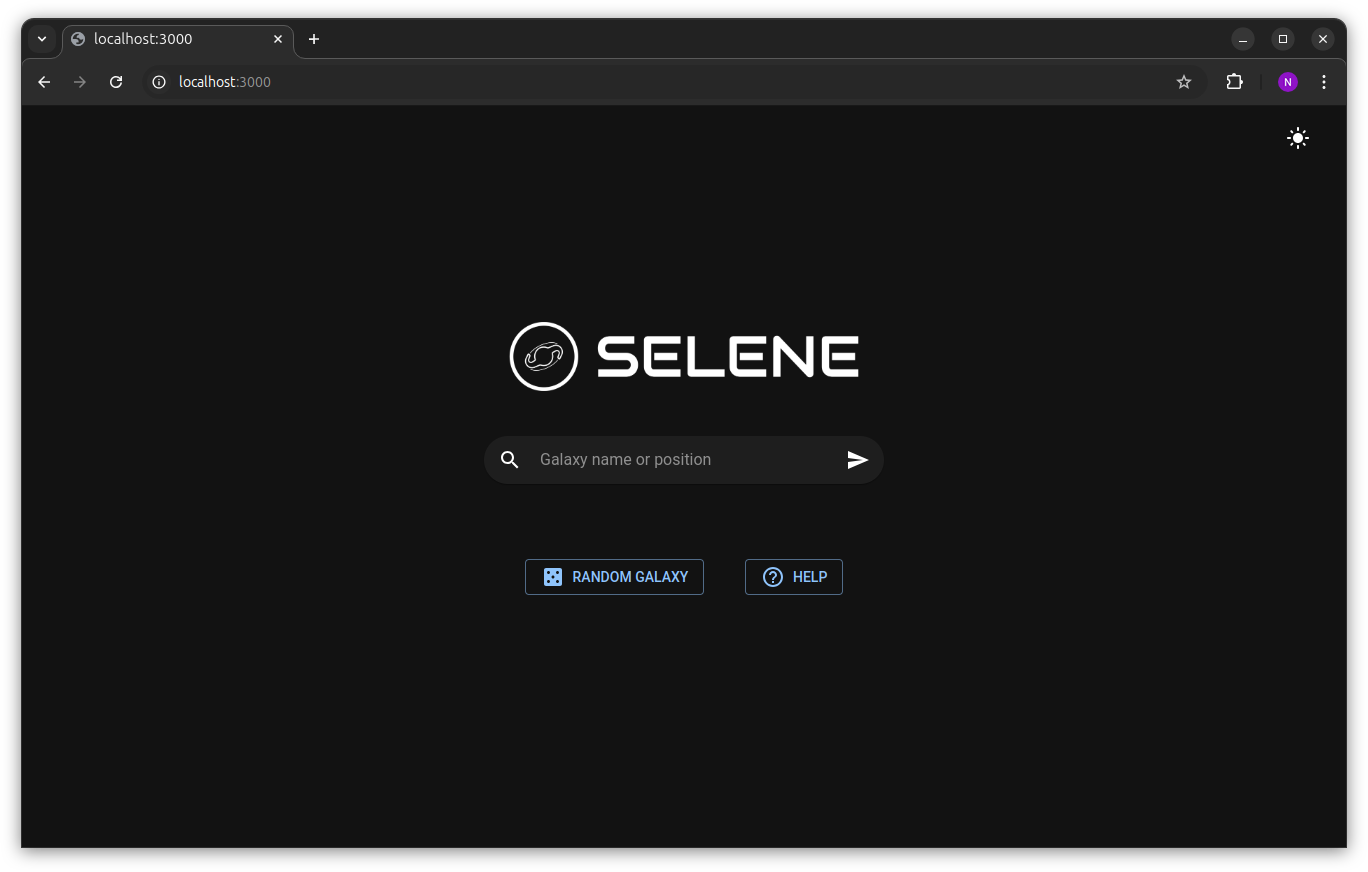
\includegraphics[width=\linewidth]{figures/screen-1.png}
  \legend{Com uma interface simples, a página inicial possui um seu centro o seu componente principal: a barra de busca. Nela, o usuário digita o nome ou posição da galáxia}
\end{figure}

\begin{figure}[!ht]
  \centering
  \caption{Página de erro para objetos não encontrados}
  \label{fig:tela-erro}
  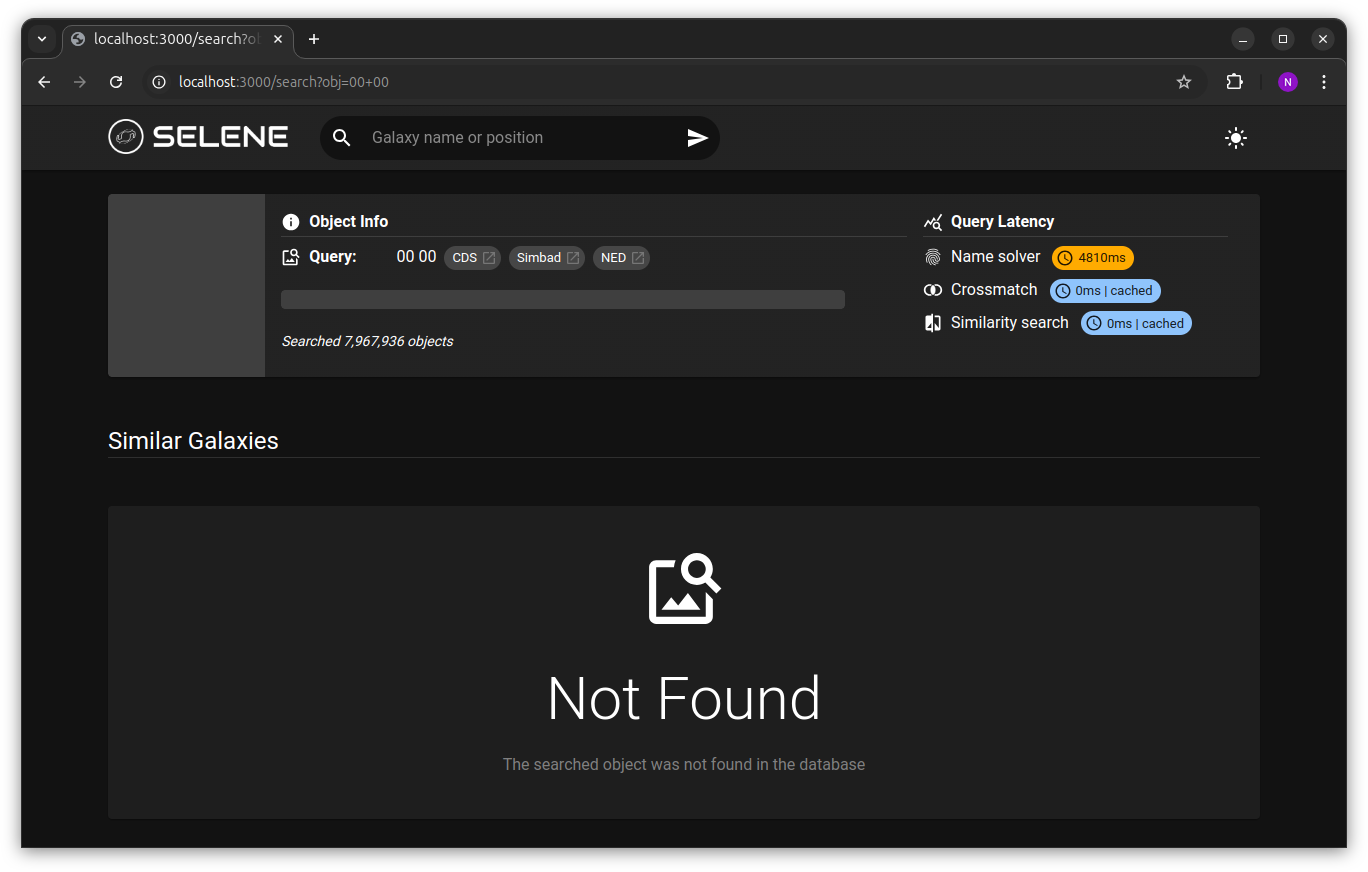
\includegraphics[width=\linewidth]{figures/screen-4.png}
\end{figure}


\begin{figure}[!ht]
  \centering
  \caption{Tela de resultados da busca}
  \label{fig:tela-resultados}
  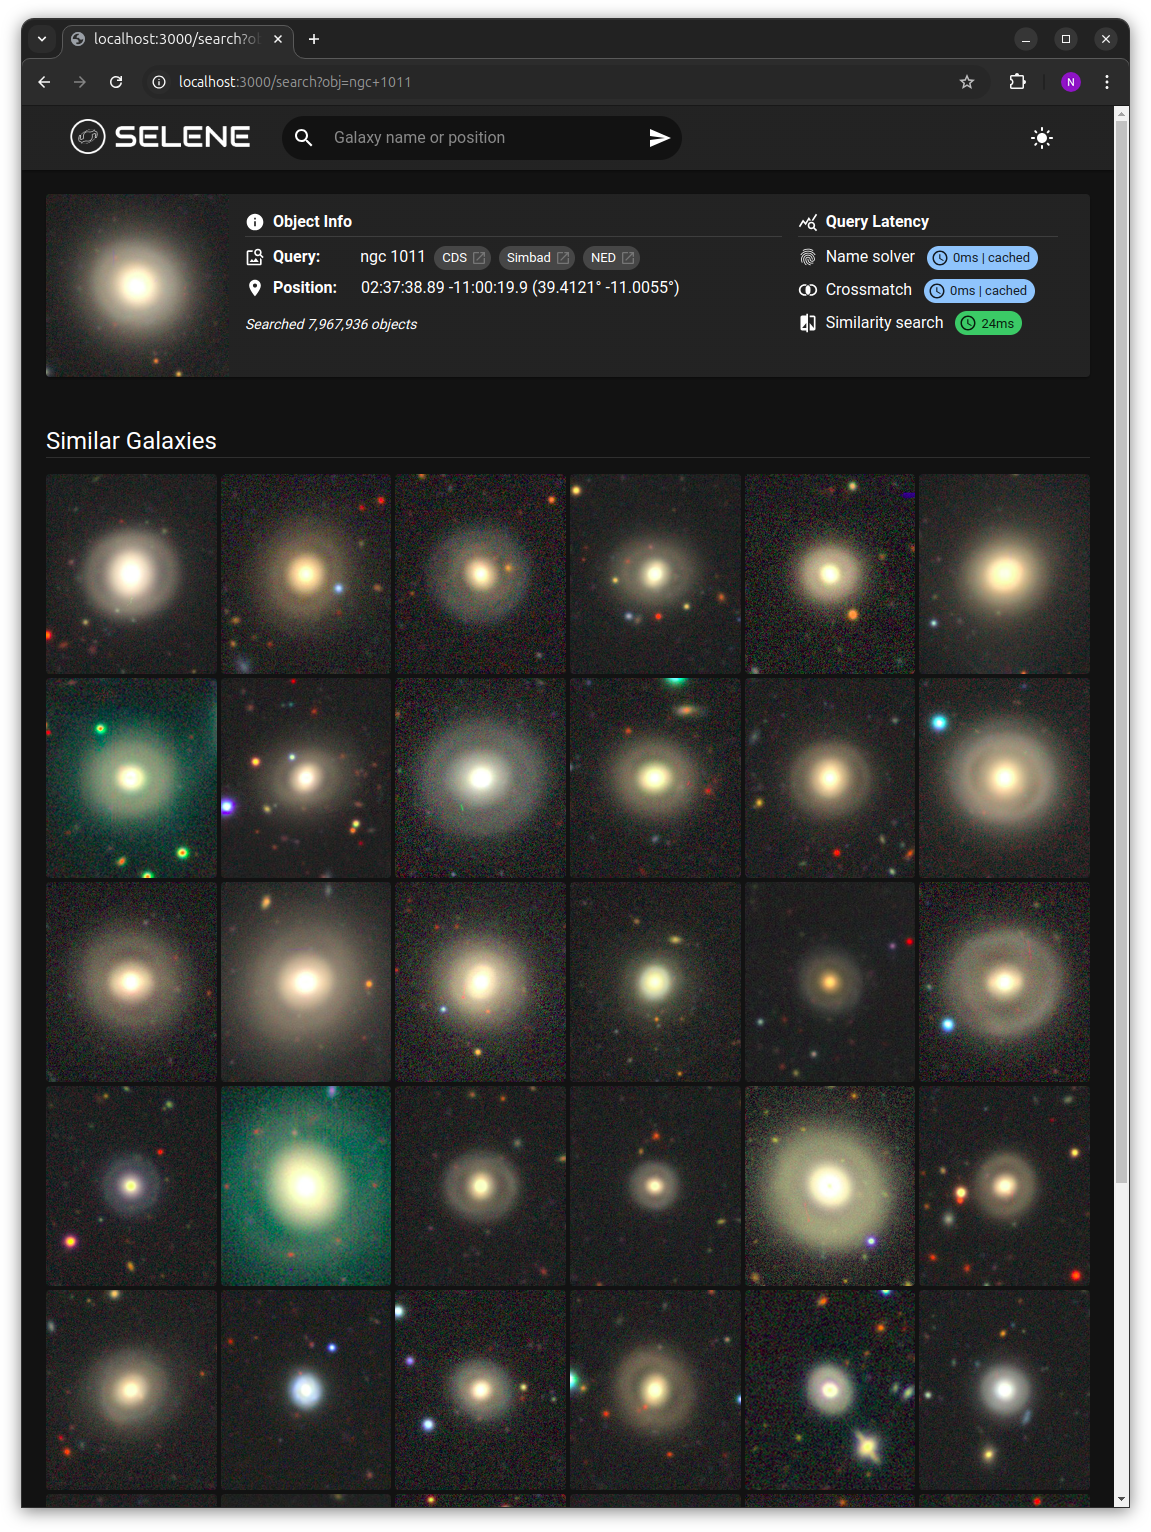
\includegraphics[width=\linewidth]{figures/screen-3.png}
  \legend{A tela de resultados exibe, no topo, um painel contendo informações adicionais da galáxia buscada e as medidas de tempo gasto em cada etapa da busca (resolução do nome, correlação e busca por similaridade). Abaixo, são mostradas todas as galáxias similares recuperadas.}
\end{figure}

\afterpage{\clearpage}



\section{Considerações Finais do Capítulo}
O capítulo apresentou os resultados obtidos no desenvolvimento e avaliação do sistema proposto, englobando três principais vertentes: a análise do modelo de aprendizado profundo (Seção \ref{sec:res-teste}), a avaliação da tarefa de recuperação de imagens (Seção \ref{sec:res-ret}) e a análise do desempenho e usabilidade do sistema de informação (Seção \ref{sec:res-sist}).

Inicialmente, na Seção \ref{sec:res-teste}, são descritas métricas como acurácia, precisão, revocação e F1-score, calculadas para diversas questões do GalaxyZoo. Os resultados evidenciam a capacidade do modelo em generalizar para novos dados e fornecer representações precisas das características morfológicas das galáxias. A análise detalhada de matrizes de confusão complementa essa avaliação, destacando o desempenho em diferentes cenários e tipos de dados. Esses resultados são fundamentais para validar a adequação do modelo ao domínio específico da astronomia.

Em seguida, a Seção \ref{sec:res-ret} explora a utilização da métrica de precisão média (mAP) para quantificar a relevância e a organização dos itens recuperados com base em consultas visuais. Os resultados mostram que o modelo alcança altos valores de mAP mesmo em cenários desafiadores, como classes desbalanceadas ou padrões visuais complexos. Exemplos de buscas realizadas para galáxias específicas, como UGC 9010 e NGC 1043, evidenciam a eficácia do sistema em identificar objetos semelhantes, reforçando sua aplicabilidade prática em contextos científicos.

Por fim, a Seção \ref{sec:res-sist} abrange os aspectos de desempenho e usabilidade. O tempo de execução das tarefas, como a busca vetorial e a resolução de nomes, é otimizado com o uso de índices e sistemas de cache. A interface gráfica é destacada por sua simplicidade e funcionalidade, permitindo a interação intuitiva de usuários com os resultados e metadados das buscas. A apresentação clara dos dados e a responsividade da aplicação garantem uma experiência de uso eficiente e acessível.



\chaptersep
